\documentclass[12pt]{article}

\usepackage{ucs}
\usepackage[utf8x]{inputenc}
\usepackage[russian]{babel}
\usepackage{array,amssymb,amsmath,graphicx,abstract,hanging,fancyhdr,float,indentfirst,blindtext,autonum}
\usepackage{mathday}

% Заполняется авторами
\setauthors{
Петров П. П.\footnote{Петров Петр Петрович, профессор, Санкт-Петербургский государственный университет},
Сидоров С. С.\footnote{Сидоров Сидор Сидорович, доцент, Московский государственный университет},
Петрова П. П.\footnote{Петрова Петра Петровна, студент, Санкт-Петербургский государственный университет}}
\settitle{Название}
\setgrant{Работа выполнена при финансовой поддержке Российского научного фонда, грант № 12-34-56789}

\begin{document}
   
	Текст с тезисами доклада оформляется в \LaTeX{} или в MS Word (см. шаблон для MS Word). Оформление текста осуществляется в соответствии с требованиями, представленными в данном файле. Все элементы, такие как рисунки, таблицы и формулы, должны быть представлены в соответствии с установленными правилами.
	
	В преамбуле необходимо задать ФИО авторов и соответствующую информацию о должности и организации с помощью команды \verb|\setauthors|. С помощью команды \verb|\settitle| задается название работы.
	По желаю указывается информация о гранте с помощью команды \verb|\setgrant|.
	
	Рисунки должны быть вставлены в текст с использованием команды \verb|\includegraphics|. Каждый рисунок должен иметь подпись, размещенную под изображением. В качестве примера приведен рис.~\ref{fig:example}.
	\begin{figure}[h!]
		\centering
		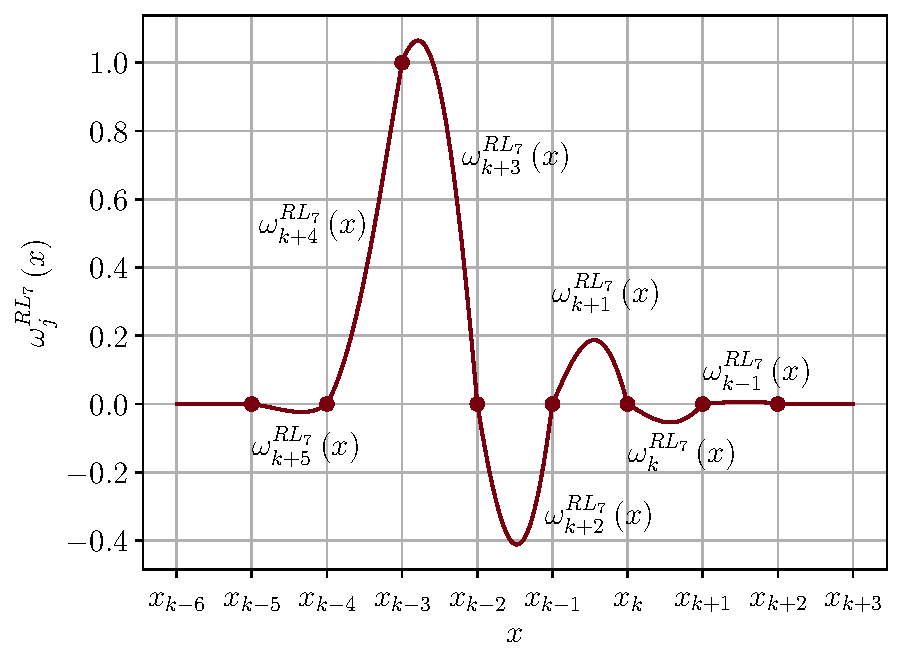
\includegraphics[width=0.55\textwidth]{figures/example.pdf} % Путь к изображению
		\caption{Пример подписи к рисунку}
		\label{fig:example}
	\end{figure}
	
	Таблицы должны быть оформлены с помощью окружения \verb|table|. Каждая таблица должна иметь номер и название, размещенное над таблицей. В качестве примера приведена таб.~\ref{tab:example}.
	\begin{table}[h!]
		\centering
		\caption{Пример таблицы}
		\label{tab:example}
		\begin{tabular}{|c|c|c|}
			\hline
			Колонка 1 & Колонка 2 & Колонка 3 \\ \hline
			Данные 1  & Данные 2  & Данные 3  \\ \hline
			Данные 4  & Данные 5  & Данные 6  \\ \hline
		\end{tabular}
	\end{table}
	
	Формулы оформляются в режиме \textit{math mode} и должны быть пронумерованы, если на них есть ссылки в тексте. Пример:
	\begin{equation}
		E = mc^2.
		\label{eq:energy}
	\end{equation}
	Формулы в тексте, такие как $a^2 + b^2 = c^2$, пишутся в строчном режиме.
	
	Ссылка на рисунок: см. рис.~\ref{fig:example}. Ссылка на таблицу: см. табл.~\ref{tab:example}. Ссылка на формулу: см. формулу~\eqref{eq:energy}. Ссылка на пункт из списка литературы:~\cite{bib:demi}.
	
    \begin{thebibliography}{1}
        \bibitem{bib:demi}
        Демидович~Б.~П. Сборник задач и упражнений по математическому анализу. М.: Издательство <<Астрель>>, 2003.
        \bibitem{bib:ro}
        Роджерс Д., Адамс Дж. Математические основы машинной графики. М.: Мир, 2001.
        \bibitem{bib:kalman}
        Kalman R. E. A new approach to linear filtering and prediction problems~// Journal of Basic Engineering. 1960. № 82 (1). P.~35--45.
    \end{thebibliography}
\end{document}
